\section{Molecular Biology Background} \label{molecular-back-sect}
The \emph{central dogma} of molecular biology explains the flow of genetic information in a biological system, that is, it states that DNA codes for RNA (\emph{transcription}), and subsequently RNA codes for proteins (\emph{translation}). This process is shown in \emph{Fig. \ref{central-dogma-pic}}. The type of RNA that is responsible for carrying messages from the nucleus to the ribosomes for the synthesis of proteins, is called \emph{messenger RNA} (mRNA) \citep{Jasny2001}. 
\vspace*{5mm}
\begin{figure}[!ht]
\begin{center}
 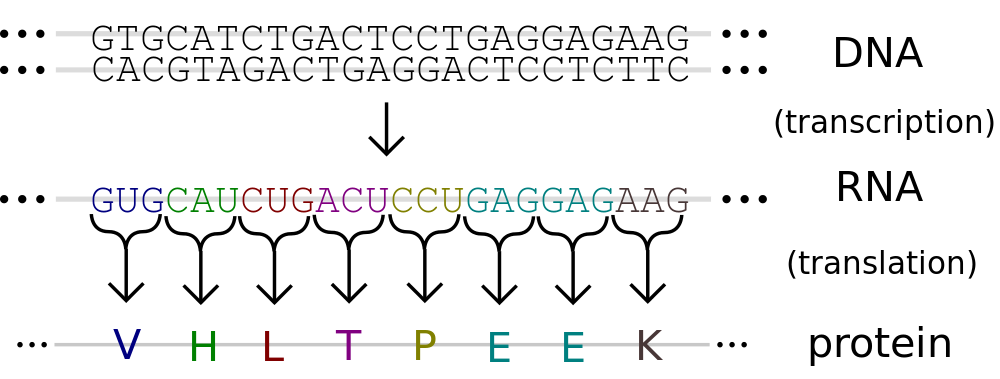
\includegraphics[scale = 0.39]{images/central-dogma3.png}
\caption{\emph{Central dogma of molecular biology. DNA is transcribed into RNA, and RNA is translated into protein (Credits: Wikipedia).}}
\label{central-dogma-pic}
\end{center}
\end{figure}

As a general rule, each cell of an organism carries the same genetic information, that is, each cell contains the exact same DNA sequence in its nucleus \citep{Jasny2001}. Yet, the human organism contains more the $200$ different cell types, which have different form and functionality. Thus, the question that arises is, what is the molecular basis for the morphological difference between cell types, \eg human blood cells and brain cells? 

The answer is that each cell expresses only specific genes (\ie makes mRNA transcripts from specific genes) that are needed for its proper function. For example, blood cells need to produce hemoglobin proteins which are needed to carry oxygen from the lungs to the tissues. On the other hand, brain cells do not need to express these specific genes for synthesizing hemoglobin proteins, but they need to express genes that synthesize proteins that are needed for specific functions of the brain.

The ability of each cell to orchestrate the synthesis of proteins by using only a specific set of genes from the \emph{genome} (\ie the whole set of genes), is termed as \emph{regulation of gene expression} \citep{Jasny2001}.

Until recently, regulation of gene expression in higher eukaryotic organisms was thought to depend only on the sequences within the DNA itself known as \emph{promoters}, and on a network of regulatory proteins, called \emph{transcription factors} (TFs) \citep{Jasny2001}. TFs are proteins that bind to specific DNA sequences, which are associated with specific genes, and facilitate of inhibit the recruitment of RNA polymerase in the promoter region of those genes \citep{Ptashne2002}. 

Recent advances in \emph{epigenomics} have suggested some other mechanisms that regulate gene expression, such as the changes of the accessibility of the DNA, e.g. \emph{histone modifications} (HMs), and \emph{DNA methylation}. Epigenomics is a relatively new scientific field in molecular biology, and it describes the study of dynamic alterations in the transcriptional regulation of a cell. We can think of the epigenome as an external layer of information onto the genomic sequence, which can be used to understand major cellular processes, such as transcription, splicing and replication \citep{Furey2012}.

Histones are proteins that act as a spool where DNA can be wrapped around them to form \emph{nucleosomes}. The combination of DNA and nucleosomes within the nucleus of eukaryotic cells is called the \emph{chromatin}. 

DNA methylation is an epigenetic mark which occurs when a methyl group is attached to the \emph{cytosine} DNA nucleotides. In mammals, DNA methylation is observed almost exclusively on cytosines in the context of CpG dinucleotides. Genome wide CpGs are depleted, but mainly near promoter regions there are clusters of CpGs, which are called CpG islands (CGIs) \citep{Bird2002}. 

%Owing to the rapid development of Next Generation Sequencing (NGS) technology, it is reasonable to expect genome sequences and other forms of high-throughput data to be measured extensively. For example, \emph{RNA-Seq} experiments \citep{Wang2009} are widely used for transcriptome profiling, i.e. measuring the set of all RNA molecules produced in a given cell or cell population (at a given time). \emph{Chip-Seq} experiments \citep{Park2009} are used to quantitatively measure and analyse protein interactions with DNA, i.e. HMs and binding of TFs. Whole-Genome Bisulphite Sequencing (WGBS) \citep{Frommer1992}, and Reduced Representation Bisulphite Sequencing (RRBS) \citep{Meissner2008}, are methods that use bisulphite treatment of DNA and allow estimation of methylation level at a single-nucleotide resolution. 

Recent research studies, assisted by whole-genome data analysis, demonstrated that gene expression and histone modifications (HMs) are well correlated, since a probabilistic model was created, which given a small number of HMs could predict gene expression \citep{Karlic2010}. Also, \citet{Benveniste2014}, using the richness of the ENCODE datasets \citep{Dunham2012}, learned a logistic regression classifier with the TFs as input features and showed that only from knowledge of TF binding patterns at promoters they could accurately predict HMs. These are only some studies that show the correlation between genetic and epigenetic mechanisms. 